\documentclass[11pt]{article}

\usepackage{graphicx,pgf}
\usepackage{tikz}

\begin{document}

\section*{Package structure}

The BEAST software is organized hierarchically into java packages.
All BEAST classes exist in packages under the dr package. Within this
namespace, there are about a dozen top-level packages:
\begin{description}
\item [{dr.app.{*}}] Application-specific code, including main class for
BEAST, BEAUti and all application specific GUI code.
\item [{dr.evolution.{*}}] Library of classes and routines describing all
the basic objects needed in import, export and manipulation of molecular
evolution data structures. No reference to XML parsing or statistical
inference procedures like MCMC. Classes in the dr.evolution.{*} packages
do not depend on classes in dr.inference.{*}, dr.evomodel.{*}, dr.evomodelxml
or dr.geo.{*}.
\item [{dr.evomodel.{*}}] Library of classes for MCMC inference on molecular
evolutionary data. This package primarily brings together the dr.evolution.{*}
and dr.inference.{*} packages.
\item [{dr.evomodelxml}] Contains XMLObjectParsers for objects in dr.evomodel.{*}
packages.
\item [{dr.evoxml}] Contains XMLObjectParsers for objects in dr.evolution.{*}
packages.
\item [{dr.geo.{*}}] Contains classes for geographical modeling.
\item [{dr.gui.{*}}] Contains classes for generic GUI objects and tasks.
Classes in the dr.gui.{*} packages do not depend on classes in dr.app.{*},
dr.inference.{*}, dr.evomodel.{*}, dr.evomodelxml or dr.geo.{*}.
\item [{dr.inference.{*}}] Contains classes for statistical inference,
\emph{without specific reference to probablistic models of molecular
evolution. }Classes in the dr.inference.{*} packages do not depend
on classes in dr.app.{*}, dr.evolution.{*}, dr.evomodel.{*}, dr.evomodelxml
or dr.geo.{*}.
\item [{dr.java16compat}]~
\item [{dr.math.{*}}] Basic numerical computing classes including mathematical
functions and optimization algorithms. Classes in this package do
not depend on classes in any other packages in BEAST.
\item [{dr.matrix}] Basic Matrix and Vector support. Classes in this package
do not depend on classes in any other packages in BEAST.
\item [{dr.stats}] A couple of basic statistics classes. Depends only on
dr.util package. 
\item [{dr.util}] Basic utility classes. Depends on no other packages.
\item [{dr.xml}] Basic XML parsing classes, \emph{without specific reference
to molecular evolution}. Depends only on dr.util package. 
\end{description}
%
\begin{figure}
\begin{centering}

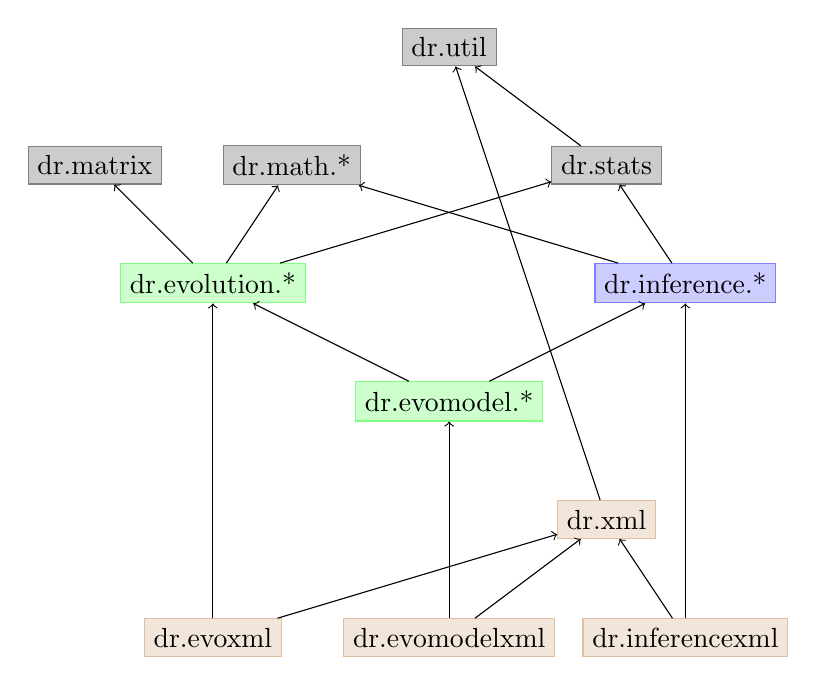
\begin{tikzpicture}[rectangle, xmlpackage/.style={draw=brown!50,fill=brown!20}, package/.style={draw=black!50,fill=black!20}, infpackage/.style={draw=blue!50,fill=blue!20}, evopackage/.style={draw=green!50,fill=green!20}]

\node[xmlpackage] (evomodelxml) at (0, -3) {dr.evomodelxml}; 
\node[xmlpackage] (evoxml) at (-3, -3) {dr.evoxml}; 
\node[evopackage] (evomodel) at (0, 0) {dr.evomodel.*}; 
\node[evopackage] (evolution) at (-3, 1.5) {dr.evolution.*}; 
\node[xmlpackage] (inferencexml) at (3, -3) {dr.inferencexml}; 
\node[infpackage] (inference) at (3, 1.5) {dr.inference.*}; 
\node[package] (stats) at (2, 3) {dr.stats}; 
\node[xmlpackage] (xml) at (2, -1.5) {dr.xml}; 
\node[package] (util) at (0, 4.5) {dr.util}; 
\node[package] (math) at (-2, 3) {dr.math.*}; 
\node[package] (matrix) at (-4.5, 3) {dr.matrix}; 

\draw [->] (inferencexml) -- (inference); 
\draw [->] (inferencexml) -- (xml); 
\draw [->] (evoxml) -- (evolution); 
\draw [->] (evoxml) -- (xml); 
\draw [->] (evomodelxml) -- (evomodel); 
\draw [->] (evomodelxml) -- (xml); 
\draw [->] (evomodel) -- (inference); 
\draw [->] (evomodel) -- (evolution); 
\draw [->] (inference) -- (math); 
\draw [->] (inference) -- (stats); 
%\draw [->] (inference) -- (xml); 
\draw [->] (evolution) -- (math); 
\draw [->] (evolution) -- (matrix); 
\draw [->] (evolution) -- (stats); 
%\draw [->] (evolution) -- (xml); 
\draw [->] (xml) -- (util); 
\draw [->] (stats) -- (util); 

\end{tikzpicture} 

\end{centering}
\caption{The dependency structure among the top-level package namespaces}
\end{figure}

\begin{figure}
\begin{centering}

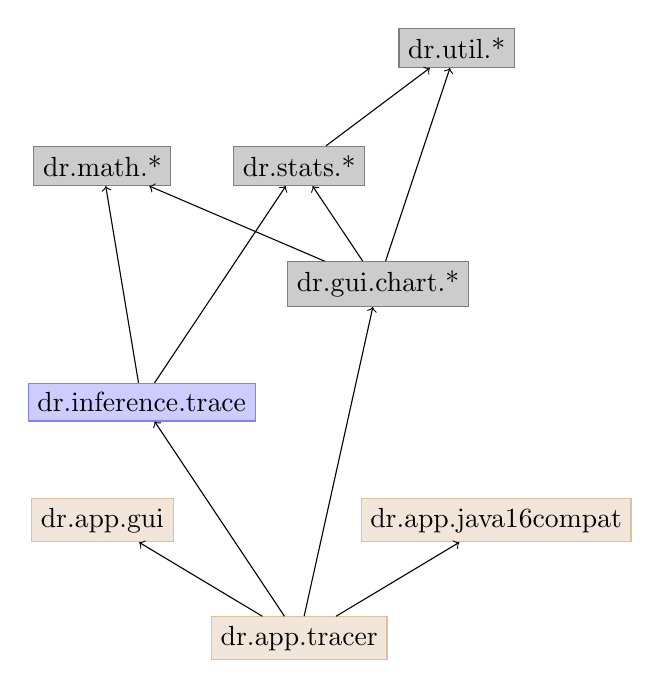
\begin{tikzpicture}[rectangle, package/.style={draw=black!50,fill=black!20}, infpackage/.style={draw=blue!50,fill=blue!20}, evopackage/.style={draw=green!50,fill=green!20}, apppackage/.style={draw=brown!50,fill=brown!20}]

\node[apppackage] (appgui) at (-2.5, -1.5) {dr.app.gui}; 
\node[apppackage] (appjava) at (2.5, -1.5) {dr.app.java16compat}; 
\node[apppackage] (tracer) at (0, -3) {dr.app.tracer}; 
\node[infpackage] (inference) at (-2, 0) {dr.inference.trace}; 
\node[package] (stats) at (0, 3) {dr.stats.*}; 
\node[package] (util) at (2, 4.5) {dr.util.*}; 
\node[package] (math) at (-2.5, 3) {dr.math.*}; 
\node[package] (gui) at (1, 1.5) {dr.gui.chart.*}; 

\draw [->] (gui) -- (util); 
\draw [->] (gui) -- (stats); 
\draw [->] (gui) -- (math); 
\draw [->] (tracer) -- (gui); 
\draw [->] (tracer) -- (appgui); 
\draw [->] (tracer) -- (appjava); 
\draw [->] (tracer) -- (inference); 
\draw [->] (inference) -- (math); 
\draw [->] (inference) -- (stats); 
\draw [->] (stats) -- (util); 

\end{tikzpicture} 

\end{centering}
\caption{The dependency structure of tracer}
\end{figure}

\end{document}
